\documentclass[journal]{IEEEtran}
\IEEEoverridecommandlockouts
% The preceding line is only needed to identify funding in the first footnote. If that is unneeded, please comment it out.
\usepackage{cite}
\usepackage{amsmath,amssymb,amsfonts}
\usepackage{algorithmic}
\usepackage{graphicx}
\usepackage{textcomp}
\usepackage{xcolor}
\usepackage{url}
\usepackage{multirow}
%\usepackage{caption}
\def\BibTeX{{\rm B\kern-.05em{\sc i\kern-.025em b}\kern-.08em
    T\kern-.1667em\lower.7ex\hbox{E}\kern-.125emX}}
\begin{document}

\title{SafeDE: A Low-Cost Hardware Solution \\ to Enforce Diverse Redundancy in Multicores \thanks{Copyright © 2017 (or current year) IEEE. Personal use of this material is permitted.  However, permission to use this material for any other purposes must be obtained by sending a request to pubs-permissions@ieee.org}}

\author{
  \IEEEauthorblockN{Francisco Bas\IEEEauthorrefmark{1}\IEEEauthorrefmark{2}, Sergi Alcaide\IEEEauthorrefmark{1}\IEEEauthorrefmark{2}, 
  Guillem Cabo\IEEEauthorrefmark{1}, Pedro Benedicte\IEEEauthorrefmark{1}, Jaume Abella\IEEEauthorrefmark{1}}\\
  \IEEEauthorblockA{\IEEEauthorrefmark{1}Barcelona Supercomputing Center (BSC)
  \\\{francisco.basjalon, sergi.alcaide, guillem.cabo, pedro.benedicteillescas, jaume.abella\}@bsc.es}
  \\\IEEEauthorblockA{\IEEEauthorrefmark{2} Universitat Polit\`{e}cnica de Catalunya (UPC)
  }
}

\maketitle

\begin{abstract}
Failure risk must be tiny
in high-integrity systems, such as those in cars, satellites and aircraft. Hence, safety measures must be deployed to avoid a single fault leading to a failure. Redundancy has been often used to address this concern, but it has been proven insufficient if a single fault can cause the same error in all redundant elements, which defeats the purpose of redundancy for error detection. Hence, to avoid this scenario, diversity is implemented along with redundancy, being lockstep execution the most popular diverse redundancy solution for computing cores. However, classic lockstep solutions have non-negligible limitations if implemented in hardware (e.g., half of the cores can only be used for redundant execution and are not even visible at user level), or in software (e.g., the software loop to enforce staggering is long and costs performance).

This paper tackles the limitations of classic lockstep solutions by 
providing an extended analysis and evaluation of
\textbf{SafeDE}, a \underline{D}iversity \underline{E}nforcement hardware module combining the short loop to enforce diversity of hardware solutions, and the non-intrusiveness of software solutions. Hence, cores can operate in lockstep mode efficiently or run independent tasks. 
In this paper, we present SafeDE and its rationale, its application to N-modular systems, its hardware and software integration, and an evaluation showing its performance and area efficiency, and its behavior in 
the presence
of faults.
\end{abstract}

\begin{IEEEkeywords}
functional safety, redundancy, diversity, faults
\end{IEEEkeywords}




\section{Introduction}

Increased autonomy levels and improved features in cars, satellites and planes lead to increasing performance demands for those systems. Existing multicores and accelerators deliver the level of performance needed. However, safety-related systems such as those in automotive, space and avionics need to meet specific safety requirements for their adoption. Those requirements are dictated by the specific safety integrity level of the functionality at hand, and are particularly demanding for the highest levels (e.g. Automotive Safety Integrity Level, ASIL, D in automotive~\cite{ISO26262}). 

A key safety requirement for the highest integrity level systems is the capability of not causing a failure due to a single fault. Those faults are normally mitigated by means of diverse redundancy~\cite{ClassicDiversity}, so that redundancy exists but it is sufficiently diverse so that a single fault affecting all replicas would cause different effects, thus allowing, at least, detecting the fault. 
%Such fault detection should allow recovering or reaching a safe state before the fault leads to a failure. 

Solutions for diverse redundancy often relate to Error Correction Codes (ECC) for storage and Cyclic Redundancy Coding (CRC) for communications~\cite{SergiIOLTS}. Computing elements (e.g. cores), instead, usually require full replication and thus, resort to dual (DMR)~\cite{Mukherjee2002,Gomaa2003,dynamic_coupled_cores} or triple modular redundancy (TMR)~\cite{Iturbe2019}. However, such redundancy is not enough and diversity is also needed to avoid that a single fault (e.g. a voltage droop or a permanent fault) affects redundant instances identically. Such diverse redundancy is achieved with lockstepping, where two (or more) identical cores execute the same software redundantly, but with some staggering among them, so that the state of the cores differs at any point in time, and thus, a fault cannot produce the same error in all redundant copies, which could go unnoticed otherwise.

Lockstepping, in the form of Dual Core LockStepping (DCLS)~\cite{infineon_aurix,STlockstep,RendundancyASILD}, is generally implemented at hardware level tying two cores together operating with few cycles of staggering (i.e. the head core executes the same software $N$ cycles ahead of the trail core). External requests are generated by one of the cores (e.g. head one), but not sent until compared to those of the other core (e.g. trail one). Upon a match, loads, stores, interrupts and any other type of request is sent, but just once (not redundantly). Responses are duplicated and delivered to both cores preserving the staggering (i.e. delivering them $N$ cycles later to the trail core). This ensures consistent states across lockstepped cores, but with some staggering to preserve diversity. Such a solution, however, makes only one of the cores be visible at software level, and precludes the user from using those cores independently.
%implies using modified cores w.r.t. those used without lockstepping, and precludes the ability to use those cores to run different software not needing lockstepping.

Light-weight software-only lockstepping has been proposed to reduce the cost of full lockstepping~\cite{SergiDFT}. Such light-weight lockstepping resorts to software redundancy, and to the existence of a software monitor enforcing staggering across redundant threads. While such a solution has been proven effective, and compatible with Commercial Off-The-Shelf (COTS) processors, it requires native lockstepping (hardware-based) for the core running the monitor, and imposes some non-negligible staggering (e.g. 100$\mu$s) to allow the monitor to collect information of the progress of redundant threads without causing too high relative interference.

Overall, both hardware-based and light software-based lockstepping pose a number of limitations to achieve diverse redundancy. This paper, addresses this challenge by proposing a different tradeoff achieving most of the benefits of both approaches with low cost.

This paper presents \emph{SafeDE}\footnote{Available as an open-source component in https://bsccaos.github.io~\cite{SafeTIWebsite}.}, a \underline{D}iversity \underline{E}nforcement hardware module providing light-lockstep support by means of a non-intrusive and flexible (programmable) hardware module that preserves staggering across cores running redundant threads, thus bringing time diversity. In particular, SafeDE is a tiny hardware module performing the same monitoring tasks as the software-only solution, but with a much lower staggering (just few cycles instead of 100$\mu$s), and without requiring native lockstepped cores. 
%Of course, while the software-only solution can be applied on COTS, SafeDE needs to be integrated in the SoC.
Compared to native hardware lockstepping, SafeDE can be integrated without modifying IP cores, thus with limited intrusiveness, and allows using cores independently instead of always in lockstep mode.
In particular, the contributions of this paper are as follows:
\begin{itemize}
\item We present SafeDE, a new hardware/software scheme for efficient, flexible and lowly-intrusive light lockstepping to achieve diverse redundancy.
\item We implement and verify SafeDE in VHDL.
\item We successfully integrate SafeDE in a space SoC based on Cobham Gaisler's NOEL-V cores, implemented in a FPGA, which is already a commercial setup for this platform reaching commercial readiness by early 2022~\cite{DeRISCjournal}.
\end{itemize}

The rest of the paper is organized as follows. Section~\ref{sec:back} provides some background. SafeDE is presented in Section~\ref{sec:dimmo} and evaluated in Section~\ref{sec:eval}. Section~\ref{sec:rel} reviews related work. Section~\ref{sec:concl} concludes this paper.


\section{Background}
\label{sec:back}

This section provides some background on the need for some form of lockstepped execution in safety-related systems, and on the existing solutions to achieve it.


\subsection{Redundancy, Diversity and Sphere of Replication}
Safety-related systems are designed so that unreasonable risk due to software faults of any kind and systematic hardware faults is avoided by design, verification and validation (V\&V). However, random hardware faults cannot be avoided and appropriate safety measures need to be deployed, such as for instance, diverse redundancy for the highest safety integrity levels (SIL for short).

There are two main approaches to achieve diverse redundancy: using diverse hardware and/or software so that replicas (e.g. redundant threads) execution is diverse in nature, or using identical hardware and software and enforcing diversity by making identical replicas run on identical hardware (but not the same hardware unit) with some staggering so that hardware state is different at any point in time. Generally, the latter is preferred since it reduces design as well as V\&V costs because only one software unit and hardware unit needs to be designed, verified and validated, rather than having to do so for multiple units. This is, for instance, the case of DCLS in Infineon AURIX multicores~\cite{infineon_aurix}.

Lockstep operation is usually implemented 
comparing only off-core activities such as load and store requests, as well as interrupts and exceptions. Thus, cores execute software redundantly with some staggering and include some buffering capabilities to store off-core requests of the head thread until they are compared with the trail thread ones, as well as to store off-core responses for the trail thread, which are delivered to the corresponding core with some staggering w.r.t. the head thread.
Other off-core resources, such as storage elements (e.g. caches, memories) and communication elements (e.g. buses, crossbars) build upon ECC and CRC to reach diverse redundancy.


\subsection{Lockstep Strands}

\begin{figure}[t!]
\centering
%\setlength{\tabcolsep}{1.0mm}
\begin{tabular}{cc}
  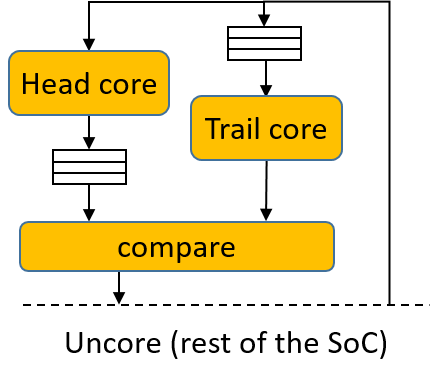
\includegraphics[width=0.40\columnwidth]{imgs/HWlockstep.png} & 
  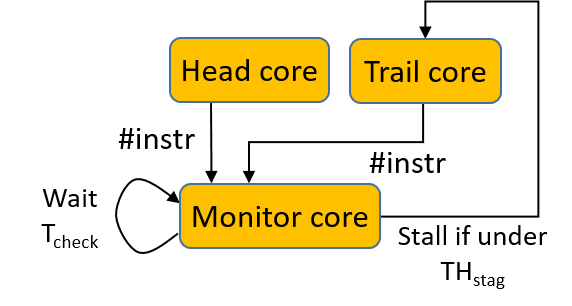
\includegraphics[width=0.50\columnwidth]{imgs/SWlockstep.png} \\
  (a) Hardware-only & (b) Software-only \\
\end{tabular}
  \caption{Schematic of hardware and software-based lockstep schemes.}
  \label{fig:HWSWlockstep}
\end{figure}

\textbf{Hardware-based tight lockstepping} builds upon two tightly coupled cores operating with identical state but with $N$ cycles of staggering, thus meaning that the head core is exactly $N$ cycles ahead in the exection of the trail core. Therefore, during fault-free operation, the trail core delivers exactly the same external signals as the head core but $N$ cycles later. This is managed with appropriate queues, as illustrated in Figure~\ref{fig:HWSWlockstep}(a). In particular, output activity of the head core needs to be stored during $N$ cycles until the trail core produces the same outputs. Then, they are compared and, if they match, the corresponding outputs are made visible out of the lockstepped cores complex, e.g. sending a load request to memory, storing data or signalling an interrupt. Externally, \emph{lockstepped cores are perceived as just one core} since only the activity generated by one of them is sent. Responses for those requests of a single core arrive just once, so they need to be replicated and delivered to both cores. In order to preserve the staggering, buffering is needed in the trail core side to keep data during $N$ cycles before delivering it to the core.
Such a scheme introduces a delay of $N$ cycles in any external access either for the outgoing requests (head core) or for the incoming responses (trail core). Nevertheless, $N$ is typically 2 or 3 cycles, so the impact of staggering is limited.

\textbf{Software-based light lockstepping} builds upon two cores able to operate independently executing different programs. Therefore, redundant threads need being created by software and scheduled accordingly into the head and trail cores which, in practice, are identical among them and inherit head or trail behavior only due to software management of their progress. The (simplified) operation, which we illustrate in Figure~\ref{fig:HWSWlockstep}(b), requires of a supporting monitor thread, which runs in another core, either in the same chip or another. For instance, this scheme has been devised to run the monitor in a processor with native hardware lockstepping, thus guaranteeing safety for the monitor, so that the monitor manages redundant threads of multiple software components running in a (likely powerful) multicore without lockstepping support. In particular, the monitor thread creates the two redundant processes and keeps the trail core stalled. Periodically, the monitor collects the number of instructions executed by the head and trail cores ($\#instr$ in the figure), and compares them. If the difference, $\#instr_{head} - \#instr_{trail}$, is above a given threshold $TH_{stag}$, then the trail core is allowed to make progress. Else, the trail core is stalled. Every $T_{check}$ cycles the monitor repeats the process. Note that $TH_{stag}$ needs to be carefully set to guarantee that, even if the head core got stalled and the trail one made progress at its maximum speed during $T_{check}$ cycles, the head core would still have a number of instructions executed higher than the trail one. If this is the case, both cores can be allowed to make progress unsupervisedly during $T_{check}$ cycles until the next monitoring check. 
There is an obvious relationship between the monitoring frequency and the staggering time: the looser the monitoring (i.e. the higher $T_{check}$) so that monitoring overhead decreases, the higher the staggering needed (i.e. the higher $TH_{stag}$). As shown in \cite{SergiDFT}, $TH_{stag}$ needs to be typically at least the maximum number of instructions that could be executed in 100$\mu$s.
Those 100$\mu$s are roughly the execution time increase that lockstepped execution will cause to let the trail core finish the execution of the trail thread after the head one does so with the head thread.



\section{SafeDE: a \underline{D}iversity \underline{E}nforcement hardware module}
\label{sec:dimmo}

This section presents SafeDE. First, we introduce the architecture of SafeDE. Then, we analyze its pros and cons in comparison with the software-only solution. Finally, we provide implementation and integration details about its deployment in a commercial space multicore.

\subsection{SafeDE Architecture}

\begin{figure}[t!]
\centering
  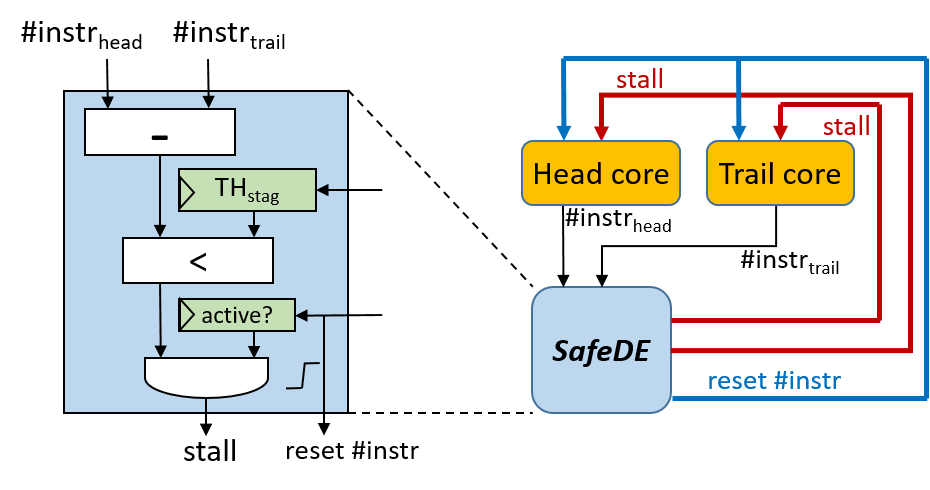
\includegraphics[width=1\columnwidth]{imgs/dimmo.png} 
  \caption{SafeDE architecture.}
  \label{fig:dimmo}
\end{figure}

SafeDE is architected to be the hardware counterpart of software-based light lockstepping. Its objective is keeping as much as possible the advantages of the software-only solution, while mitigating its limitations, which we discuss in next subsection. For that purpose, SafeDE is devised as a tiny module coupled to each pair of cores potentially needing to operate lockstepped. This is illustrated in Figure~\ref{fig:dimmo}. As shown, SafeDE requires the instruction count values of the lockstepped cores, as well as an interface signal to stall the trail core. SafeDE subtracts the number of instructions of the trail core from those of the head core, $\#instr_{head} - \#instr_{trail}$, as in the case of the software-only solution, and compares the difference against a staggering threshold, $TH_{stag}$. Only when the head core is not sufficiently ahead of the trail core, and SafeDE is active, a stall signal is sent to the trail core, which must be used to stall the core whenever set. Such stall can be achieved, for instance, stalling all stages (e.g. blocking pipeline latches), stalling only the commit stage, or stalling only the fetch stage, to name few alternatives. 

\textbf{SafeDE parameters}. SafeDE has four configuration registers: $TH_{stag}$, $active$, $CritSec1$ and $CritSec2$. 
%\textcolor{red}{SA: Later on we describre that we use 3 registers}
\begin{itemize}
\item $TH_{stag}$ stands for the minimum number of instructions that the head core must be ahead of the trail core. Typical values are few instructions, very much in line with hardware-based tight lockstepped cores. Note that this value is several orders of magnitude lower than that for software-only solutions. 
\item $active$ signal indicates whether SafeDE is active or not. If reset, SafeDE produces no effect. Else, SafeDE operates normally. Whenever the parameter is set to 1 (input signal raised), lockstep operation is possible, which is practically controlled by the other registers.
\item $CritSec1$ and $CritSec2$ registers indicate whether core 1 (head) and core 2 (trail) have entered the ``critical'' code region to be executed in lockstep mode. 
%a reset signal is sent to $\#instr_{head}$ and $\#instr_{trail}$ so that they are reset synchronizedly.
\end{itemize}

\textbf{SafeDE operation}. SafeDE is, at some point, inactive ($active=0$). No action is performed by SafeDE until $active$ is set, regardless of the values of the other registers. 
Eventually, SafeDE is programmed setting $TH_{stag}$ as needed, and then $active$ is set.
Once $active=1$, $CritSec1$ and $CritSec2$ are reset, and SafeDE awaits for the corresponding activation of $CritSec1$ and $CritSec2$.  
$CritSec1$ and $CritSec2$ are set by core1 and core2 respectively when they reach their critical section. The first core entering the critical section will take the role of the head core. Whenever the head core sets its $CritSec$ register, its instruction count ($\#instr_{head}$) resets and starts counting the committed instructions. If the trail core activates its $CritSec$ register before the staggering is large enough ($\#instr_{head} - \#instr_{trail} < TH_{stag}$), the stall signal is sent to the trail core.
%Whenever $CritSec1$ is set, the head core gets its instruction count reset ($\#instr_{head}$) and executes normally. Whenever $CritSec2$ is set, the trail core gets its instruction count reset ($\#instr_{trail}$) and waits for (1) the head core to enter its critical code region ($CritSec1$ is set), and (2) for the staggering to be large enough. If $CritSec1$ is not set, or $\#instr_{head} - \#instr_{trail} < TH_{stag}$, then a stall signal is sent to the trail core.
%Since the stall signal for the trail core is ANDed with $active$, it is zero and no action is performed. 
%Whenever $active$ is set, $\#instr_{head}$ and $\#instr_{trail}$ in the head and trail cores respectively are reset. 
%Then, if SafeDE detects that the $\#instr_{head} - \#instr_{trail} < TH_{stag}$, then a stall signal is sent to the trail core. 
%Note that this occurs automatically when SafeDE is activated since $\#instr_{head}$ and $\#instr_{trail}$ are both reset simultaneously. 
%This allows the head core to gain some staggering w.r.t. the trail core. 
As soon as the staggering is enough, the stall signal is reset and the trail core starts execution. Note that SafeDE performs the subtraction $\#instr_{head} - \#instr_{trail}$ and the comparison against $TH_{stag}$ every cycle. This allows using very low values for $TH_{stag}$ as opposed to the software-only solution. Despite performing such action every cycle, note that $\#instr_{head}$ and $\#instr_{trail}$ barely change every cycle (e.g. they do not change or just are incremented by up to very few instructions). Therefore, activity due to the subtraction and comparison is tiny since most of input signals remain constant, and hence, signal switching occurs seldom.
Whenever the head core reaches the end of its critical section, it resets $CritSec1$. From that point onwards, SafeDE allows the trail core execute without any stall until it also finishes its critical region ($CritSec2$ is also reset).


\textbf{Software process}. To use SafeDE, end users, either by themselves or with the support from an appropriate API, need to create the two redundant processes, schedule them to the head and trail cores, and keep them stopped (e.g. with $SIG\_STOP$ signals). Then, SafeDE needs being configured and set to active state. Finally, both redundant processes need to be set to active (e.g. with $SIG\_CONT$ signals).


\subsection{Features and Limitations Analysis}

SafeDE offers a different tradeoff to that of the software-only solution. Next, we detail its main features and limitations along with whether they are common with the software-only solution in \cite{SergiDFT} or not.

\subsubsection{SafeDE features}
\begin{itemize}
\item \textbf{Low cost}. As shown before, SafeDE is a tiny module offering support to enforce staggering to achieve diverse redundancy. SafeDE releases the system from having to allocate a task with strict timing requirements (e.g. executing at a very specific frequency), as needed in the case of the software-only solution. 
\item \textbf{Low staggering}. By being implemented in hardware and monitoring instruction counts from the head and trail cores constantly, SafeDE can guarantee diversity even if staggering is low (e.g. $TH_{stag}$ set to few instructions). This is also an advantage w.r.t. the software-only solution, which requires heavier activities by being conducted by software means, reading remote registers, issuing interrupts to stall/resume execution in a core, etc., so needing a much higher staggering than SafeDE.
\item \textbf{Flexibility}. SafeDE can be enabled/disabled at will, thus being usable at very fine granularity. Still, the granularity is dictated by the ability of the software to create the redundant processes and stop/resume them at start up. Hence, flexibility is high, but the granularity at which SafeDE can be used is similar to that of the software-only solution.
\item \textbf{Low intrusiveness}. SafeDE needs cores to export few signals for its integration, thus being much less intrusive than hardware-based tight lockstepping. In particular, SafeDE needs cores to expose their instruction count register for monitoring purposes, an appropriate stall signal to stall the trail core whenever needed, and the reset signal for the instruction count register. 
%Thus, these are minor changes to the cores. 
Differently, the software-only solution does not require any hardware change, although it may require modifications into the operating system to allow reading the instruction count register from remote cores. SafeDE, instead, does not need any such operating system change.
\end{itemize}

\subsubsection{SafeDE limitations}
\begin{itemize}
\item \textbf{Non-null intrusiveness}. Hardware changes required by SafeDE are minor, but they are not null, so differently to the software-only solution, SafeDE cannot be deployed on COTS ASIC multicores.
\item \textbf{Limited applicability}. SafeDE, as well as the software-only solution, needs that redundant processes execute exactly the same instructions so that software does not diverge. Otherwise, SafeDE (and the software solution) would become ineffective. For instance, this implies that SafeDE should not be used for functions whose execution path depends on random choices or physical address bits, which could follow different paths across redundant processes. For the former case, SafeDE can be used if identical random values are enforced across processes (e.g. providing the same random number stream with a software-implemented pseudo-random number generator initialized identically for both processes). Similarly, SafeDE cannot be used for parallel applications if the execution path and the instruction count may vary across redundant threads due to synchronization (e.g. different order to access sequential code regions). In any case, such limitation is analogous to that of the software-only solution. Also, SafeDE (and software solutions) cannot be applied for processes with some form of I/O accesses, since those accesses need to be performed only once generally, but redundant processes would perform those accesses twice.
\item \textbf{Limited diversity}. Physical diversity is achieved by running redundant processes in different cores. SafeDE, as well as the software only solution, provides also time diversity. However, other sources of \emph{common cause failures} (i.e. identical failures in both cores due to a single fault), such as for instance those related to physical degradation of specific gates of the processor need other types of diversity (e.g. layout diversity) that cannot be achieved by any external monitor, either hardware (SafeDE) or software.
\item \textbf{SafeDE hardening}. Since faults could also affect SafeDE, it must be hardened to meet sufficiently low failure rates or, simply, deployed with physical diverse redundancy, as for tight lockstepped cores (e.g. using the scheme in Figure~\ref{fig:HWSWlockstep}(a) but for SafeDE instead of the cores). 
\end{itemize}

\subsubsection{Scope of applicability}
Due to the limited applicability of SafeDE, as in the case of software-only solutions, SafeDE cannot be applied to all software but to code regions. For instance, if data is read from a sensor, processed and sent to an actuator, SafeDE and software only solutions can be applied to the processing part only. If full (end-to-end) diverse redundancy is needed, native (hardware-based) tight lockstepping support is needed, as explained in \cite{SergiDFT}. In particular, at least two cores need to be paired with hardware-based tight lockstepping to execute sensor and actuator interactions. However, the most performance hungry part of the execution (i.e. data processing) can be managed with SafeDE. Thus, deployments where only two cores provide hardware-based tight lockstepping, and the rest support light lockstepping with SafeDE would be highly efficient. For instance, an 8-core multicore could be deployed with (a) 4 pairs of hardware-based tight lockstepped cores, thus offering only 4 user-visible cores; (b) 1 pair of hardware-based tight lockstepped cores and 6 non-lockstepped cores, thus offering 7 user-visible cores, but only up to 1 concurrent task running with diverse redundancy; or (c) 1 pair of hardware-based tight lockstepped cores and 6 cores paired with SafeDE, thus offering 7 user-visible cores, and supporting up to 4 concurrent tasks running with diverse redundancy. 
%While other hybrid combinations would be possible (e.g. 2 pairs of hardware-based tight lockstepped cores and 4 non-lockstepped cores), examples (a), (b) and (c) already allow understanding the flexibility offered by SafeDE.



\subsection{Implementation and Integration}
\label{sec:integ}

\begin{figure}[t!]
\centering
  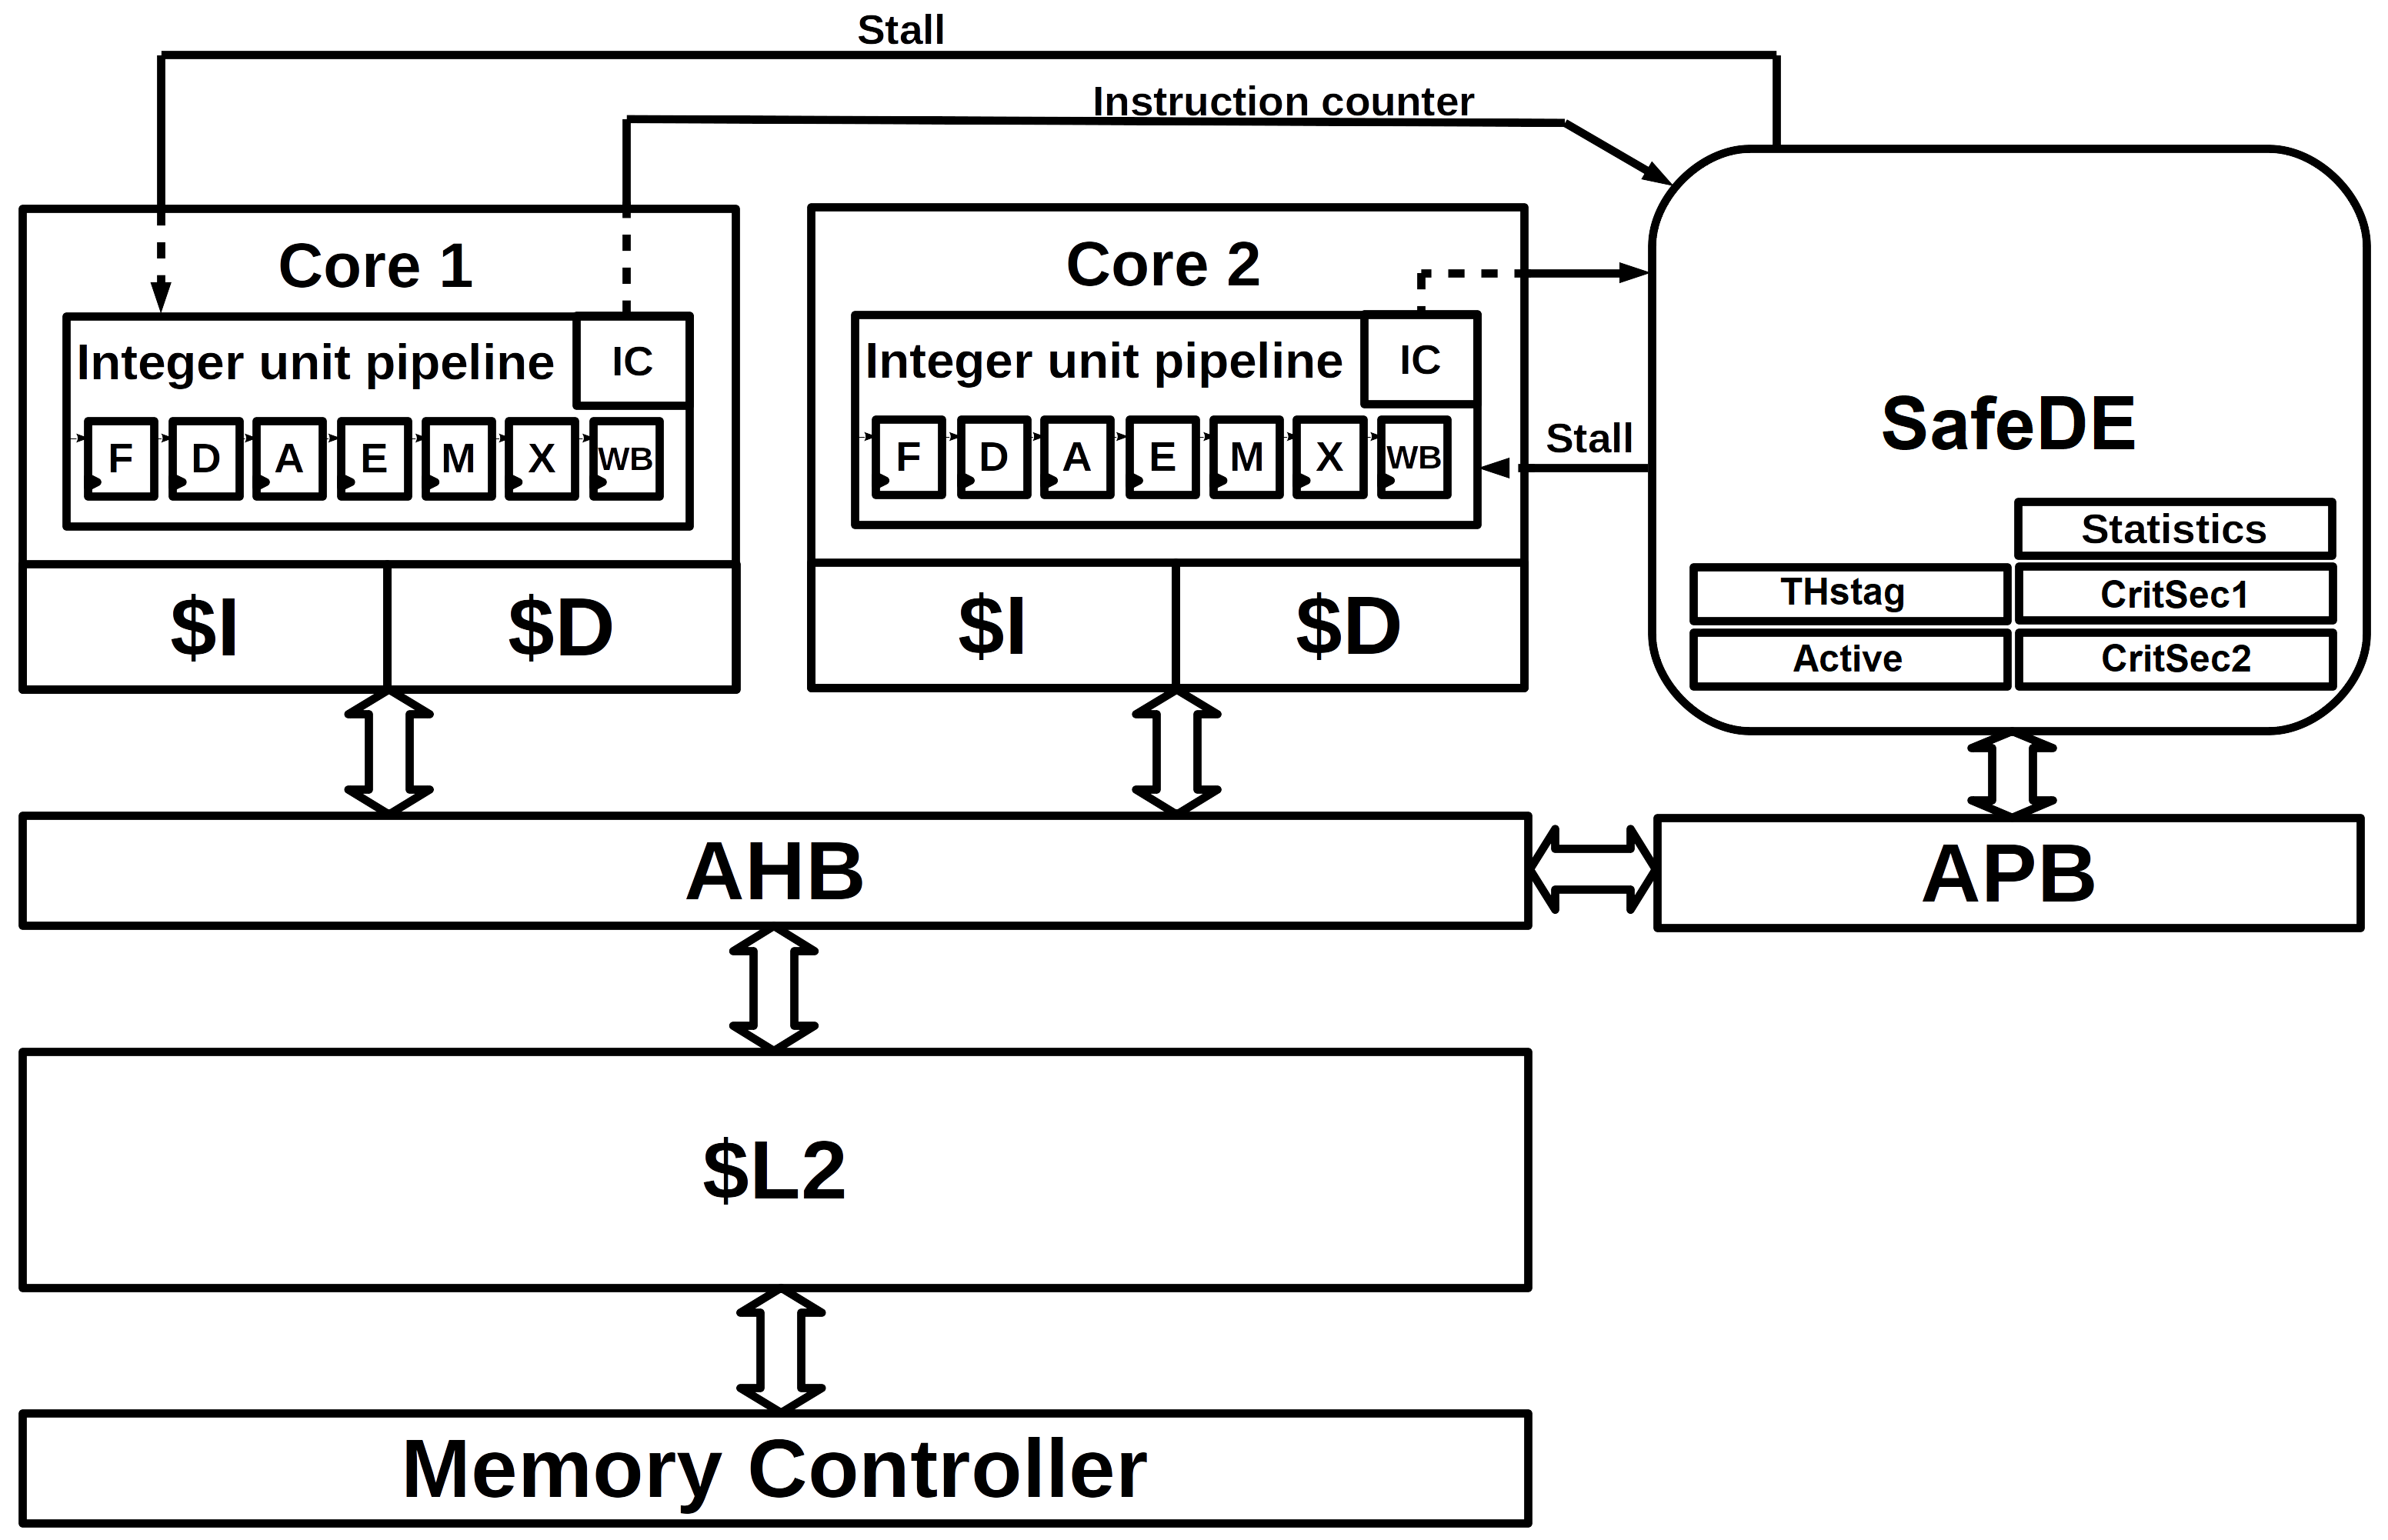
\includegraphics[width=1\columnwidth]{imgs/system.png} 
  \caption{High-level representation of SafeDE integrated into the system.}
  \label{fig:system}
\end{figure}

To prove its feasibility, SafeDE has been integrated and evaluated in an industrial space product, namely the RISC-V based Cobham Gaisler NOEL-V MultiProcessor System on Chip (MPSoC). In this platform, Cobham Gaisler provides an integrated set of reusable VHDL IP cores centered around common on-chip buses. The buses of the selected MPSoC are based on the standard AMBA 2.0. SafeDE is designed in VHDL as one of the reusable Gaisler IP cores. 

\subsubsection{System on Chip}
The SoC where SafeDE is tested comprises 2 RISC-V based 64-bit dual-issue 7-stages pipeline NOEL-V cores. Apart from the main 128 bits Advanced High-performance Bus (AHB), another AHB is used for debugging purposes. For low bandwidth peripherals as SafeDE, an Advanced Peripheral Bus (APB) is employed.

Each core includes private L1 Data and Instruction caches. Data L1 caches are write-through with a write-no-allocate policy. A shared L2 cache is connected to the main shared AMBA AHB, and to the memory controller. 


\subsubsection{Integration}
SafeDE is integrated as an APB slave connected to the system through a standard APB interface. Thus, SafeDE is highly portable and can be easily embedded into any system implementing an APB interface.

Apart from the APB standard signals, SafeDE needs a few interconnections with the cores. The instruction counter of each core has to be mapped as an input. Instruction counters are employed to calculate the total number of instructions commited by each core and compute its difference. SafeDE has one output to stall the trail core. That SafeDE output is ORed with an internal pipeline signal in charge of holding the pipeline (i.e. keeping constant the pipeline registers values). Therefore, when SafeDE needs to stall the trail core, SafeDE can stall that core just asserting the respective output. 
Therefore, the only modifications needed in the cores correspond to exporting the instruction counter\footnote{Note that virtually any processor implements instruction and cycle performance monitoring counters.} value to make it visible to SafeDE, and placing the OR gate needed let SafeDE set the pipeline stall signal whenever needed.
Figure \ref{fig:system} shows a high-level representation of SafeDE integrated into the system.


\subsubsection{Configuration and operation}
SafeDE is controlled and configured by means of four internal registers. Each register is mapped to a specific SoC memory position. The first one, $TH_{stag}$, is used to configure the minimum staggering. The second one, $active$, is used to enable/disable SafeDE. Each of the two remaining registers, $CritSec1$ and $CritSec2$, is coupled with one core and set to 1 when the respective core starts the critical section (i.e. with a store instruction to this register in the application), and set to 0 when it finishes its execution. This procedure allows SafeDE to synchronize both cores at the beginning of the critical section, even if they do not start simultaneously, as explained before. Neither of the cores assumes the role of trail or head core until its critical section starts. 
%The first core writing its SafeDE enable register is set as the head core during that execution.

%A detection mechanism was also designed to ensure that both cores reach the critical section within a specified time. Otherwise, an interruption is raised.

In addition to these four registers, SafeDE has also several registers to gather some statistics such as maximum staggering, minimum staggering, times that the trail core has been stalled, how many cycles the trail core has been stalled, committed instructions by each core, etc. The connection of SafeDE to the MPSoC allows SafeDE registers to be written and read through usual load and store operations. 


\section{Evaluation}
\label{sec:eval}

We evaluate SafeDE by synthesizing the RISC-V multicore SoC into a Xilinx Kintex UltraScale KCU105 evaluation kit.

%\subsection{Simulation and verification}
\subsection{Validation}
%\subsubsection{Simulation example}
%A view extracted from the system simulation exposing the SafeDE working mechanism is found in Figure \ref{fig:chronogram}. First, at cycle 1, the chronograph shows how the lower threshold ($TH_{min}$) is crossed (instructions difference becomes smaller than 10), and the signal to stall the trail core (core2) is raised. The trail core remains stalled until the head core computes at least one instruction (just one cycle in this example). Later, at cycle 5, the upper threshold ($TH_{max}$) is crossed (instruction difference becomes larger than 15). Again, the head core (core1) is stalled until the trail core executes at least one instruction (until cycle 8 in this example).

%\subsubsection{Verification}
%To further evaluate the correct functioning of SafeDE once implemented in the FPGA, two registers that store the minimum and the maximum staggering that both cores reach during the execution are integrated. During the execution of the TACLe benchmarks set, in no case, the staggering is lower or higher than the values allowed by the thresholds.

%\begin{figure}[t!]
%\centering
%  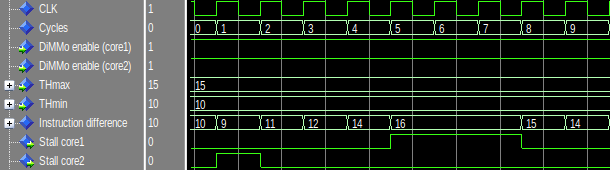
\includegraphics[width=1\columnwidth]{imgs/chronogram.png} 
%  \caption{Piece of a chronogram extracted from a simulation of the system executing the TACLe benchmark Fac and with SafeDE active forcing a controlled diversity.}
%  \label{fig:chronogram}
%\end{figure}

In order to validate the correct functioning of SafeDE once implemented in the FPGA, we have added a register recording the lowest staggering observed between the head and tail cores. We have used the TACLeBench benchmark suite~\cite{taclebench}, which is a set of open-source self-contained benchmarks intended to evaluate basic functionalities in real-time systems. They have been chosen because, since their source files already include inputs hardcoded, they can be easily compiled and run on a baremetal setup without any support to read data from files. Moreover, since some of the benchmarks are quite simple (i.e. execution times range between some hundreds and some millions of cycles), they ease debugging and validation on a simulated environment.
Therefore, we have set the staggering to 10 cycles, $TH_{stag} = 20$, and recorded the lowest staggering observed across all benchmarks. Our experiments confirm that the actual staggering has never been below this number of cycles, hence providing evidence that SafeDE works as expected.


\subsection{Execution time overhead}


%\subsubsection{Execution time overhead in a set of TACLe benchmarks}
To elucidate the impact of SafeDE in terms of computational overhead, we have run the TACLeBench benchmarks in three different scenarios:
\begin{itemize}
\item \emph{Isolation}: only one core executes the benchmark and the other core remains idle. 
\item \emph{Redundancy without diversity}: two different cores execute the same benchmark without any control mechanism. 
\item \emph{Redundancy with diversity} enforced by SafeDE: SafeDE guarantees that the minimum staggering, $TH_{stag}$, is never exceeded. 
\end{itemize}

In our evaluation, we have set $TH_{stag} = 20$ for illustration purposes. Note that the lowest value that must be used for the staggering relates to the pipeline depth of the core (7 stages in the specific platform used) given that the instructions difference is obtained using committed instructions. Hence, using a pipelined core, it could occur that, by the time staggering is about to fall below the threshold and the trail core stalled (i.e. its commit stage is stalled), the pipeline of the trail core could be executing some common instructions to those of the head core in some of the stages if the staggering is too low. Thus, we have set the threshold to be high enough so that this cannot happen in a pipeline with 7 stages and a pipeline width of 2 instructions.

%Large instruction difference between thresholds limits the overhead because it is less likely for each core to be stalled. Since this is not a limitation for most applications, we chose a conservative difference. Concretely, SafeDE is configured with $TH_{min} = 20$ and $TH_{max} = 1000$.

Note that, by using a light-lockstep approach, redundant processes are generated loading binaries twice (one for each core) in different memory segments.
%Unlike the tight lockstep approach, both cores execute different memory segments containing the same benchmark, so both executions run isolated. 
We execute each benchmark 1,000 times and use the average cycle count for each one for our evaluation to discount the effect of small variations due to, for instance, delays caused by DRAM refreshes. In any case, absolute variations observed are always in the order of few tens of cycles.

\begin{figure}[t!]
\centering
  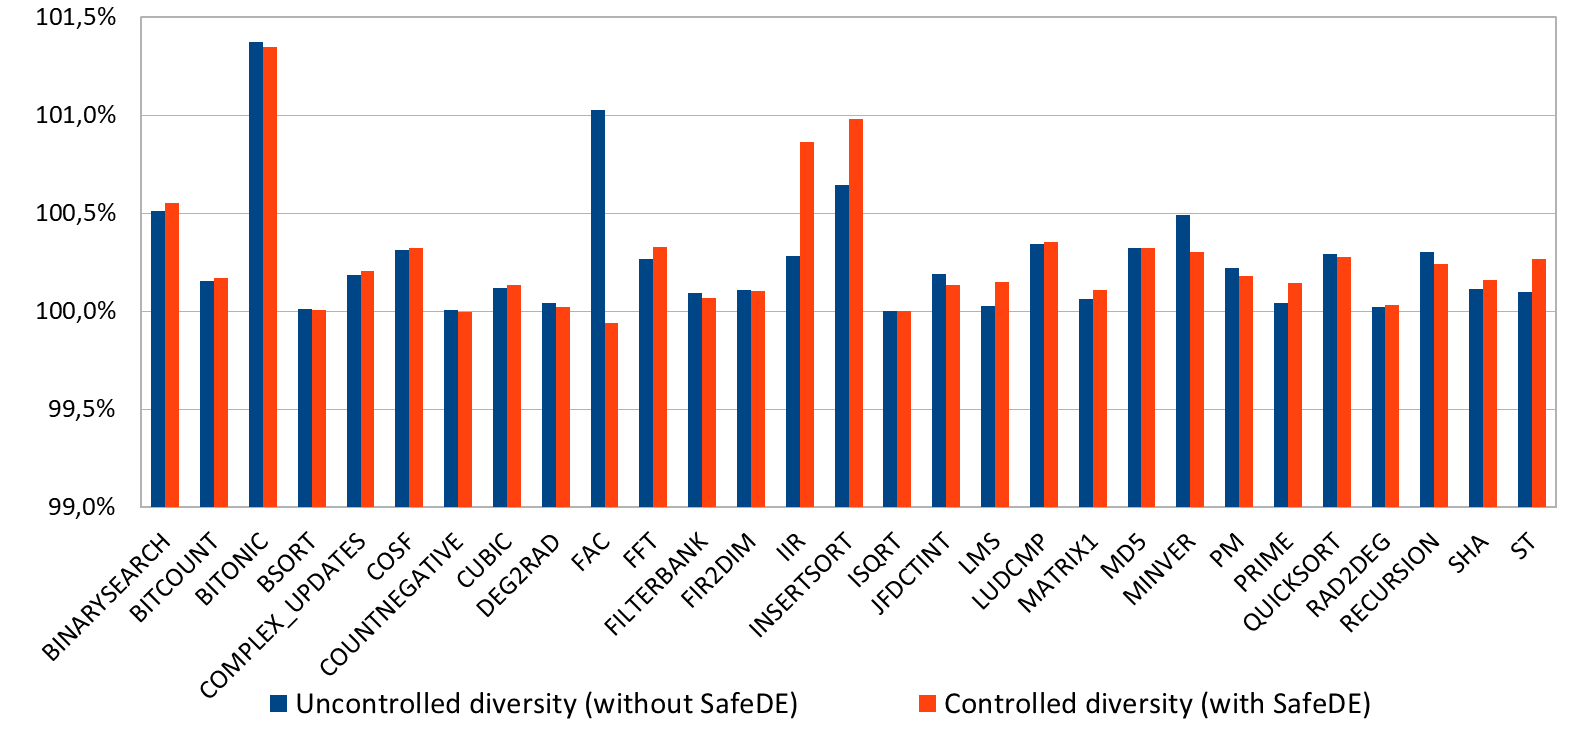
\includegraphics[width=1\columnwidth]{imgs/tacle_results.png} 
  \caption{Execution time of different TACLeBench benchmakrs normalized w.r.t. their execution time in isolation. Each benchmark is executed 1,000 times.}
  \label{fig:tacle_results}
\end{figure}

Results are shown in Figure~\ref{fig:tacle_results}. As shown, in all the cases, the execution time overhead with SafeDE w.r.t. the execution time in isolation and in two cores without SafeDE is negligible. In particular, SafeDE causes an execution time degradation in most of the cases below 0.5\%, and up to 1.3\% in one case (\texttt{BITONIC} benchmark) w.r.t. the execution time in isolation. If we compare it against the redundant execution without enforcing diversity, execution time degradation is generally below 0.1\% (in some cases performance even marginally improves), and up to 0.6\% for \texttt{IIR} benchmark.

%The biggest difference is found during the execution of the benchmark IIR and is smaller than a 0.6\%. The average overhead across all benchmarks w.r.t isolation execution is 0.17\%.

In some cases, minor performance variations between the isolation and redundant versions of the programs are observed, being those differences neither caused by interference between redundant threads, nor by SafeDE operation itself. Instead, those variations are caused by the initial core state (e.g. branch predictor state), or changes in instruction cache behavior due to changes in the memory alignment of the binaries with and without thread redundancy.
%effects related to instruction pipelining and memory alignment into instruction cache lines of the code may cause minor performance variations between the isolation and redundant versions of the programs not related to interference between redundant threads or SafeDE operation itself. 
In the case of \texttt{FAC} benchmark, since it is a small benchmark (around 700 instructions only), these tiny effects have a visible impact in relative terms (e.g. 1\% execution time increase without SafeDE and 0.1\% decrease with SafeDE). 

%As shown, in the case of \texttt{FAC} benchmark, the execution time with SafeDE is slightly lower than in isolation. Note that this behavior occurs systematically across the 1,000 runs performed for this benchmark. We have analyzed the source of this behavior in a simulated environment and found out that this benchmark is quite sensitive to the combination of pipelining effects and the state of the branch predictor. This benchmark, which is fact is a factorial program, performs frequent conditional branches. The first branches as well as the last ones may be missed. Hence, depending on how interference in the bus occurs, delays to access L2 cache (e.g. to write through data) may cause increased execution time or may avoid following mispredicted paths. This explains why uncontrolled diversity (without SafeDE) experiences interference in the bus that increases execution time, whereas controlled diversity (with SafeDE) avoids following some mispredicted paths. In any case, these are minor effects that would typically cancel out, but have an accumulative effect in our baremetal setup.

%We can see that for benchmarks Fac and Countnegative, the execution time happens to be smaller during the execution with SafeDE than in the execution in isolation. These results are explained due to a difference in the internal state of the core running in isolation and the cores running with SafeDE. This difference is caused both by synchronization mechanisms that have to be applied when two cores are active and by the SafeDE configuration previous to the execution. In these two benchmarks, this difference in the internal state affects the branch predictor behavior and causes systematically small differences in every iteration that increase the execution time in isolation w.r.t. the execution time with SafeDE. Since the overhead caused by SafeDE is minimal, the increase in the execution time due to a slower branch predictor in isolation is significant enough to end up being bigger than that overhead produced by SafeDE.

Overall, as expected, execution time increase can be regarded as negligible since the staggering threshold can be set very low (20 cycles in our evaluation), thus far below the 100$\mu$s, which correspond to many thousands of cycles, imposed by the software-only solution~\cite{SergiDFT}.


%\subsubsection{Relation between instruction difference between thresholds and execution time overhead}
%To infer how the instruction difference between both thresholds affects computational overhead, we have run the entire set of TACLe benchmarks, one after the other, 100 times and measured the total exectution time. We have done this 30 times and modifying the thresholds each time by keeping the $TH_{min}$ constant to 20 instructions, whereas $TH_{max}$ is increased. Time overhead for each pair $TH_{max}-TH_{min}$ can be seen in Figure \ref{fig:thresholds_overhead}. In the Y-axis is represented the time overhead of executing the entire TACLe benchmarks set with SafeDE w.r.t the execution time of the entire TACLe benchmarks set with only one core.

%\begin{figure}[t!]
%\centering
%  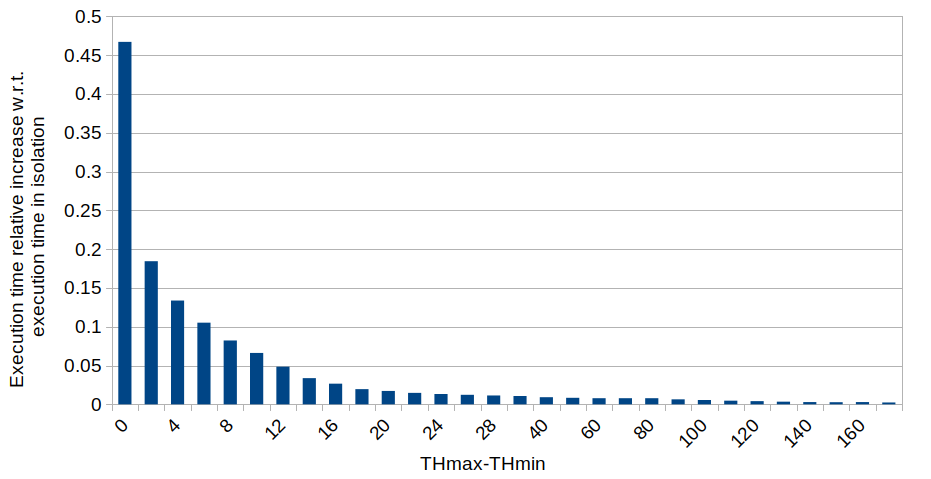
\includegraphics[width=1\columnwidth]{imgs/thresholds_overhead.png} 
%    \caption{Total execution time overhead with SafeDE of the whole set of TACLe benchmakrs w.r.t. its execution in isolation. For each run, the entire set of TACLe benchmarks are executed 100 times with the specified threshold configuration.}
%  \label{fig:thresholds_overhead}
%\end{figure}

%Overhead at low values of $TH_{max}-TH_{min}$ is above 45\%. However, overhead quickly decreases when the instruction difference between both thresholds increase. At 30 instruction distance, overhead is only 1\%, and at 170 instructions difference, overhead further reduces to 0.2\%. The more significant the difference between both thresholds, the smaller the overhead. Therefore, we can conclude that if SafeDE is used with an appropriate difference of instructions between both thresholds, the overhead becomes negligible.


\subsection{Hardware costs}

We synthesized our RISC-V design using the Vivado 2018 Toolchain and target the FPGA present in the Xilinx UltraScale KCU105. The overall cost of SafeDE implementation is 261 LUTs and 417 registers, whereas the entire SoC uses approximately 114,000 LUTs and 74,000 registers. Each core uses around 38,000 LUTs and 17,000 registers. Hence, SafeDE is a low-cost component representing just 0.23\% of the entire SoC LUTs and 0.56\% of entire SoC registers. SafeDE uses just 0.35\% of the LUTs of the pair of cores it manages, and 1.23\% of their registers. These numbers can be further improved by removing all the logic devoted to gather statistics. 


\section{Related Work}
\label{sec:rel}

\begin{table}[t!]
\centering
%\setlength{\tabcolsep}{1.0mm}
\caption{Classification of redundant execution techniques.}
\label{table:Fault-Tolerant-Classification}
\begin{tabular}{|c|c|c|l|}
\hline
Strategy & Target & Diversity & \multicolumn{1}{c|}{Approaches} \\ \hline
\multirow{5}{*}{HW} & \multirow{3}{*}{CPU} & Yes (tight) & ~\cite{STlockstep,Iturbe2019,relaxing_criticallity} \\ \cline{3-4}
 &  & Yes (light) & ~\textbf{Our approach (low staggering)} \\ \cline{3-4}
 &  & No & ~\cite{Rotenberg1999,SMTredundancy,Mukherjee2002,Gomaa2003,dynamic_coupled_cores,on_demand_redundancy} \\ \cline{2-4}
 & \multirow{2}{*}{GPU} & Partially & ~\cite{SergiDATE} \\ \cline{3-4}
 &  & No & ~\cite{instruction_replication_gpu,Jeon2012,Swapcodes,Nathan2015} \\ \hline
\multirow{4}{*}{SW-Only} & \multirow{3}{*}{CPU} & Yes (light) & ~\cite{SergiDFT} (high staggering)\\ \cline{3-4}
 &  & \multirow{2}{*}{No} & ~\cite{Haas2017,Shye2007,Scales2010,Reis2005}, \\ %\cline{2-4}
 &  &    & ~\cite{So2018,Alhakeem2015,Shye2009,Mushtaq2013} \\ \cline{2-4}
 & \multirow{2}{*}{GPU} & Partially & ~\cite{SergiIOLTS} \\ \cline{3-4}
 &  & No & ~\cite{softwareapproaches_gpgpureliability,inter-intra-workgroup,Jain2019,Vargas2018} \\ \hline
\end{tabular}
\end{table}



Some solutions to implement redundancy relate to Redundant Multi-Threading in a multi-threaded core~\cite{SMTredundancy,Rotenberg1999}, as well as across different cores~\cite{Mukherjee2002,Gomaa2003,dynamic_coupled_cores}, and even building on partial redundancy~\cite{relaxing_criticallity,on_demand_redundancy}. Unfortunately, none of those solutions guarantees diversity, either by reusing the same hardware inside the core, or by failing to impose any staggering at all. 
Some software-only solutions for CPUs enforce redundancy by compiler means, building on transactional memory, or creating monitoring threads~\cite{Reis2005,So2018,Haas2017,Mushtaq2013,Shye2007,Shye2009}.
However, none of those solutions is effective to capture single faults affecting all redundant units (a.k.a. Common Cause Faults, CCFs).

The particular case of GPUs has been addressed to provide redundancy with hardware support~\cite{inter-intra-workgroup,Jeon2012,Swapcodes,Nathan2015} or relying only on software solutions~\cite{softwareapproaches_gpgpureliability,inter-intra-workgroup,Jain2019}, but not providing diversity. Both redundancy and diversity have been achieved in GPUs with~\cite{SergiDATE} and without hardware support~\cite{SergiIOLTS}. Unfortunately, those solutions are GPU specific and cannot be extrapolated to CPUs.

Some designs provide native tight lockstep, such as ST Microelectronics SPC56XL70~\cite{STlockstep} and Infineon AURIX processor family~\cite{infineon_aurix}, which provide DCLS. Analogously, some Arm Cortex-R5 designs extend lockstep to triple-core implementations~\cite{Iturbe2019,paper1}.
Since errors are only detected when erroneous data is exposed beyond the core sphere, some authors have proposed extensions to shorten error detection time~\cite{TCAD}, and to enhance recovery~\cite{DATEcheckpointing}. 
In any case, as explained before, tight lockstep makes half of the cores non-visible to the user, thus diminishing flexibility drastically.

Reviriego et al.~\cite{DivDMR} show that, for some dual diverse redundant designs, it is possible perform recovery if the erroneous output can be identified without needing to compare it against a fault-free reference, which allows to tell what of the two diverse redundant designs delivers the correct output.

Flexible diverse redundancy on CPUs has been implemented so far with software-only solutions~\cite{SergiDFT} but, as explained before, staggering imposed is large, which leads to non-negligible performance degradation if tasks duration is short (e.g. between 100$\mu$s and 1ms). 
Our work aims at leveraging very limited hardware cost to mitigate such limitation of software-only solutions, thus complementing existing solutions (see Table~\ref{table:Fault-Tolerant-Classification}).


{\color{magenta}
%ASIL D compliant ST Microelectronics SPC56XL70~\cite{STlockstep} and Infineon AURIX processor family~\cite{infineon_aurix} implement DCLS, whereas some Arm Cortex-R5 designs implement Triple-Core Lockstep~\cite{Iturbe2019}, but fail to provide enough performance for AD systems~\cite{paper1}.
%Some improvements shorten time-to-detection for errors~\cite{TCAD} or enhance recovery processes~\cite{DATEcheckpointing}, but do not improve performance.

%Another family of solutions for high-performance CPUs builds upon thread redundancy inside a single core~\cite{SMTredundancy,Rotenberg1999}, or across cores~\cite{Mukherjee2002,Gomaa2003,dynamic_coupled_cores}, even with only partial redundancy~\cite{relaxing_criticallity,on_demand_redundancy}. However, those solutions require hardware support for thread synchronization, and differently to DCLS, do not guarantee diversity.
%Some SW-only solutions exist for CPUs~\cite{Reis2005,So2018,Haas2017,Mushtaq2013,Shye2007,Shye2009}, introducing redundancy at compiler level, building on transactional memory or creating a monitoring process to check for errors, among other solutions. However, none of them guarantees execution staggering of both redundant threads, so CCFs may cause the same error in both threads, which may lead to a failure.

%Analogous solutions for accelerators (e.g. GPUs or the Kalray MPPA family) have been proposed, either with hardware support~\cite{inter-intra-workgroup,Jeon2012,Swapcodes,Nathan2015} or with software-only support~\cite{softwareapproaches_gpgpureliability,inter-intra-workgroup,Jain2019}, but none of them guarantees diversity. Some preliminary solutions guarantee diversity to some extent for GPUs either with~\cite{SergiIOLTS} or without hardware support~\cite{SergiDATE}.

%However, to the best of our knowledge, no software-only solution guarantees diversity for CPUs, which is the challenge we address in this work, as summarized in Table~\ref{table:Fault-Tolerant-Classification}.
}



\section{Conclusions}
\label{sec:concl}


Safety-related systems must implement diverse redundancy for the highest integrity functionalities to avoid CCFs. Tight lockstepping is the \emph{de facto} solution for CPUs, but it makes half of the cores not visible at user level, so significant performance is lost when none or few high-integrity tasks are run. Light-weight lockstepping has been proposed recently to overcome such limitation and gain flexibility. However, existing solutions build on slow software feedback loops that impose large staggering and require an additional core to run the monitoring process.

This paper introduces SafeDE, a tiny module implementing light-weight lockstepping with a very short feedback loop (e.g., 20 cycles), hence causing negligible performance impact, and not needing any additional core since SafeDE itself controls the feedback loop. Our results show that SafeDE incurs both negligible performance degradation (0.5\% on average) and hardware overheads ($\approx$0.5\% extra SoC area) w.r.t. to a non-redundant industrial SoC, and effectively captures all CCFs that would also be captured by tight lockstep execution.


\color{black}


\section*{Acknowledgements}
This work has received funding from the European Union's Horizon 2020 research and innovation programme under grant agreement no. 871467. 
This work has also been partially supported by the Spanish Ministry of Science and Innovation under grant PID2019-107255GB-C21/AEI/10.13039/501100011033.


\bibliographystyle{plain}
\bibliography{biblio}

\end{document}
